\subsection{Kafka}
	All'interno del progetto ThiReMa viene fatto uso della piattaforma Apache Kafka per trasportare e trasformare i dati provenienti dai dispositivi, verso le altre componenti del sistema.
	\newline
	Per questo progetto è stato utilizzato un broker singolo, ma nulla vieta, in un futuro, di estendere l'architettura creando un cluster composto da più broker.
	\newline
	\newline
	I principali topic che sono stati creati e che vengono utilizzati dalle vari componenti sono:
	\begin{itemize}
		% Un topic per domarli...
		\item un topic per ogni gateway, all'interno del quale vengono riversati i dati raccolti dai dispositivi associati;
		% ...un topic per trovarli...	
		\item un topic per ogni gateway, nel quale vengono inviate le configurazioni per i gateway stessi;
		% ...un topic per ghermirli...		
		\item un topic in cui vengono inseriti i messaggi di alert quando uno o più sensori superano delle 
		soglie stabilite.
		% ...e nel buio incatenarli.
	\end{itemize}
	Per effettuare il rilascio di questa componente è stato realizzato un apposito file docker-compose (al cui interno sono presenti anche le altre componenti) che imposta automaticamente gli indirizzi e le porte in cui ascoltare e ricevere i messaggi. Quindi per modificare le configurazioni del broker kafka o per aggiungerne altri è sufficiente modificare il file docker-compose.yml fornito.
	\newline
	Di seguito viene riportato un piccolo estratto del file di configurazione.

		\begin{figure}[H]
			\centering
			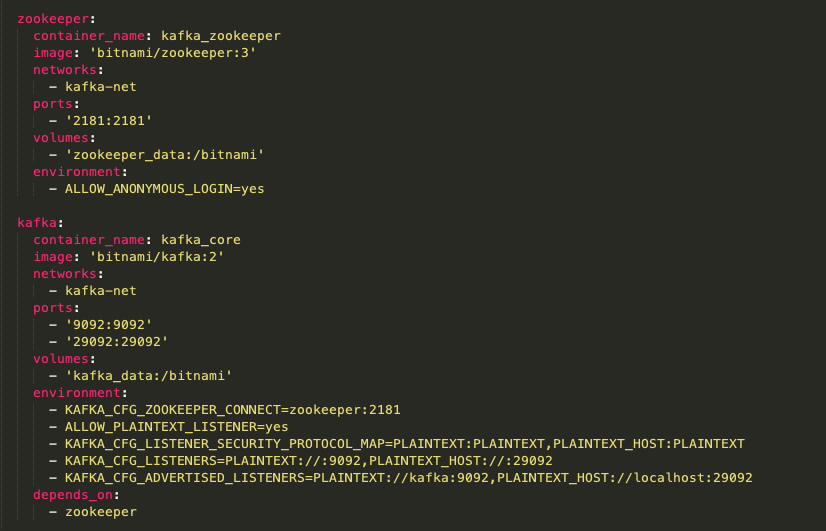
\includegraphics[scale=0.470]{res/images/estrattoKafka_dockerCompose.png}
			\caption{Estratto del file docker-compose.yml in cui viene impostato Kafka}
			\label{Immagine 1}
		\end{figure}
	\subsubsection{Estensione}
		\paragraph{Aggiungere un broker Kafka}
		Per aggiungere un ulteriore broker è necessario modificare il file docker-compose.yml. 
		All'interno del file è necessario creare un nuovo service in cui è necessario copiare il broker preesistente modificandone il nome del servizio, il nome del container e la mappatura della porte, prestando attenzione a mantenere le stesse porte interne.
		Per poterlo utilizzare è necessario solamente specificare le nuove porte assegnate. all'interno delle componenti.
		Per modificare le configurazioni si consiglia di seguire il link seguente: \url{https://github.com/bitnami/bitnami-docker-kafka}   
	